% TODO(team): Maintain the proposal text and its supporting citations.
%%%%%%%%%%%%%%%%%%%%%%%%%%%%%%%%%%%%%%%%%%%%%%%%%%%%%%%%%%%%%%%%%%%%%%%%%%%%%%%%
% Template for USENIX papers.
%
% History:
%
% - TEMPLATE for Usenix papers, specifically to meet requirements of
%   USENIX '05. originally a template for producing IEEE-format
%   articles using LaTeX. written by Matthew Ward, CS Department,
%   Worcester Polytechnic Institute. adapted by David Beazley for his
%   excellent SWIG paper in Proceedings, Tcl 96. turned into a
%   smartass generic template by De Clarke, with thanks to both the
%   above pioneers. Use at your own risk. Complaints to /dev/null.
%   Make it two column with no page numbering, default is 10 point.
%
% - Munged by Fred Douglis <douglis@research.att.com> 10/97 to
%   separate the .sty file from the LaTeX source template, so that
%   people can more easily include the .sty file into an existing
%   document. Also changed to more closely follow the style guidelines
%   as represented by the Word sample file.
%
% - Note that since 2010, USENIX does not require endnotes. If you
%   want foot of page notes, don't include the endnotes package in the
%   usepackage command, below.
% - This version uses the latex2e styles, not the very ancient 2.09
%   stuff.
%
% - Updated July 2018: Text block size changed from 6.5" to 7"
%
% - Updated Dec 2018 for ATC'19:
%
%   * Revised text to pass HotCRP's auto-formatting check, with
%     hotcrp.settings.submission_form.body_font_size=10pt, and
%     hotcrp.settings.submission_form.line_height=12pt
%
%   * Switched from \endnote-s to \footnote-s to match Usenix's policy.
%
%   * \section* => \begin{abstract} ... \end{abstract}
%
%   * Make template self-contained in terms of bibtex entires, to allow
%     this file to be compiled. (And changing refs style to 'plain'.)
%
%   * Make template self-contained in terms of figures, to
%     allow this file to be compiled. 
%
%   * Added packages for hyperref, embedding fonts, and improving
%     appearance.
%   
%   * Removed outdated text.
%
%%%%%%%%%%%%%%%%%%%%%%%%%%%%%%%%%%%%%%%%%%%%%%%%%%%%%%%%%%%%%%%%%%%%%%%%%%%%%%%%

\documentclass[letterpaper,twocolumn,10pt]{article}
\usepackage{usenix2019_v3}

% to be able to draw some self-contained figs
\usepackage{tikz}
\usepackage{amsmath}
\usepackage{graphicx}

% inlined bib file
% Bibliography is maintained in references.bib.

%-------------------------------------------------------------------------------


%-------------------------------------------------------------------------------
\begin{document}
%-------------------------------------------------------------------------------

%don't want date printed
\date{}

% make title bold and 14 pt font (Latex default is non-bold, 16 pt)
\title{\Large \bf COMPSCI 512 Project Proposal}

%for single author (just remove % characters)
\author{
{\rm Haoyu Wang}\\
hw418@duke.edu
\and
{\rm Yuquan Hu}\\
yh511@duke.edu
\and
{\rm Tian Xia}\\
tx55@duke.edu
% copy the following lines to add more authors
% \and
% {\rm Name}\\
%Name Institution
} % end author

\maketitle

%-------------------------------------------------------------------------------
% \begin{abstract}
% %-------------------------------------------------------------------------------
% Your abstract text goes here. Just a few facts. Whet our appetites.
% Not more than 200 words, if possible, and preferably closer to 150.
% \end{abstract}


%-------------------------------------------------------------------------------
\section{Topic Overview}
%-------------------------------------------------------------------------------
We propose a fault-tolerant cooperative video storage and streaming system for a group of machines with limited, heterogeneous storage. Rather than keeping every video on every machine or relying on a central video server, the system divides each video into small, hash-verified segments and distributes them among participating peers. A viewer retrieves any missing segments directly from one or more peers, allowing the group to maintain a video library larger than any individual machine can store.

The main challenge is to provide responsive playback despite limited capacity and unreliable peers. Machines may disconnect or have different storage, latency, and upload bandwidth; popular videos can also overload a few peers. Our system will therefore choose where segments are stored based on demand and peer availability, retrieve urgent segments from multiple peers before their playback deadlines, and repair lost copies after failures. It will also limit the storage and upload burden imposed on any one participant.
%-------------------------------------------------------------------------------
\section{Related Work}
%-------------------------------------------------------------------------------
\paragraph{Storage placement.} We separate metadata management from block storage: a small metadata service records video manifests and segment locations, while peers transfer segments directly. To use storage efficiently, the system will keep extra replicas of popular or early video segments and use lower-cost erasure coding for less urgent segments. This follows the recovery-speed versus storage-overhead tradeoff studied by HACFS \cite{xia2015tale}.

\paragraph{Playback scheduling.} Hsu and Hefeeda show that selecting peers to deliver video segments before playback deadlines is computationally difficult, and propose a practical approximation algorithm \cite{hsu2010quality}. Inspired by this work, our client will use a lightweight heuristic: prioritize the nearest playback deadline, prefer peers with sufficient estimated bandwidth, balance requests across peers, and retry another peer if a transfer fails.

\paragraph{Fault tolerance.} Raft provides a practical method for replicating a consistent metadata log despite controller failure \cite{ongaro2014raft}. We will use a three-node Raft group only for metadata and task records, never for video bytes. For peer failures, the system will distinguish temporary disconnection from permanent data loss before creating a repair copy, avoiding unnecessary repair traffic.

\paragraph{Background scheduling.} MapReduce demonstrates how distributed observations can be aggregated into a batch decision \cite{dean2004mapreduce}. In our system, peers periodically report request counts, free storage, and online time. A MapReduce-inspired job aggregates these reports into popularity and availability estimates, which the placement scheduler uses to issue copy, repair, and eviction tasks. This batch process is separate from the latency-sensitive playback scheduler.

Our contribution is to combine these techniques into a cooperative video system that jointly considers playback urgency, storage limits, peer availability, and fair resource use.
% Footnotes should be places after punctuation characters, without any
% spaces between said characters and footnotes, like so.%
% \footnote{Remember that USENIX format stopped using endnotes and is
%   now using regular footnotes.} And some embedded literal code may
% look as follows.

% \begin{verbatim}
% int main(int argc, char *argv[]) 
% {
%     return 0;
% }
% \end{verbatim}

% Now we're going to cite somebody. Watch for the cite tag. Here it
% comes. Arpachi-Dusseau and Arpachi-Dusseau co-authored an excellent OS
% book, which is also really funny, and
% Waldspurger got into the SIGOPS hall-of-fame due to his seminal paper
% about resource management in the ESX hypervisor

% The tilde character (\~{}) in the tex source means a non-breaking
% space. This way, your reference will always be attached to the word
% that preceded it, instead of going to the next line.

% And the 'cite' package sorts your citations by their numerical order
% of the corresponding references at the end of the paper, ridding you
% from the need to notice that, e.g, ``Waldspurger'' appears after
% ``Arpachi-Dusseau'' when sorting references
% alphabetically. 

% It'd be nice and thoughtful of you to include a suitable link in each
% and every bibtex entry that you use in your submission, to allow
% reviewers (and other readers) to easily get to the cited work, as is
% done in all entries found in the References section of this document.

% Now we're going take a look at Section, but not before
% observing that refs to sections and citations and such are colored and
% clickable in the PDF because of the packages we've included.

%-------------------------------------------------------------------------------
% \section{Floating Figures and Lists}
% \label{sec:figs}
% %-------------------------------------------------------------------------------


% %---------------------------
\begin{figure}
\begin{center}
    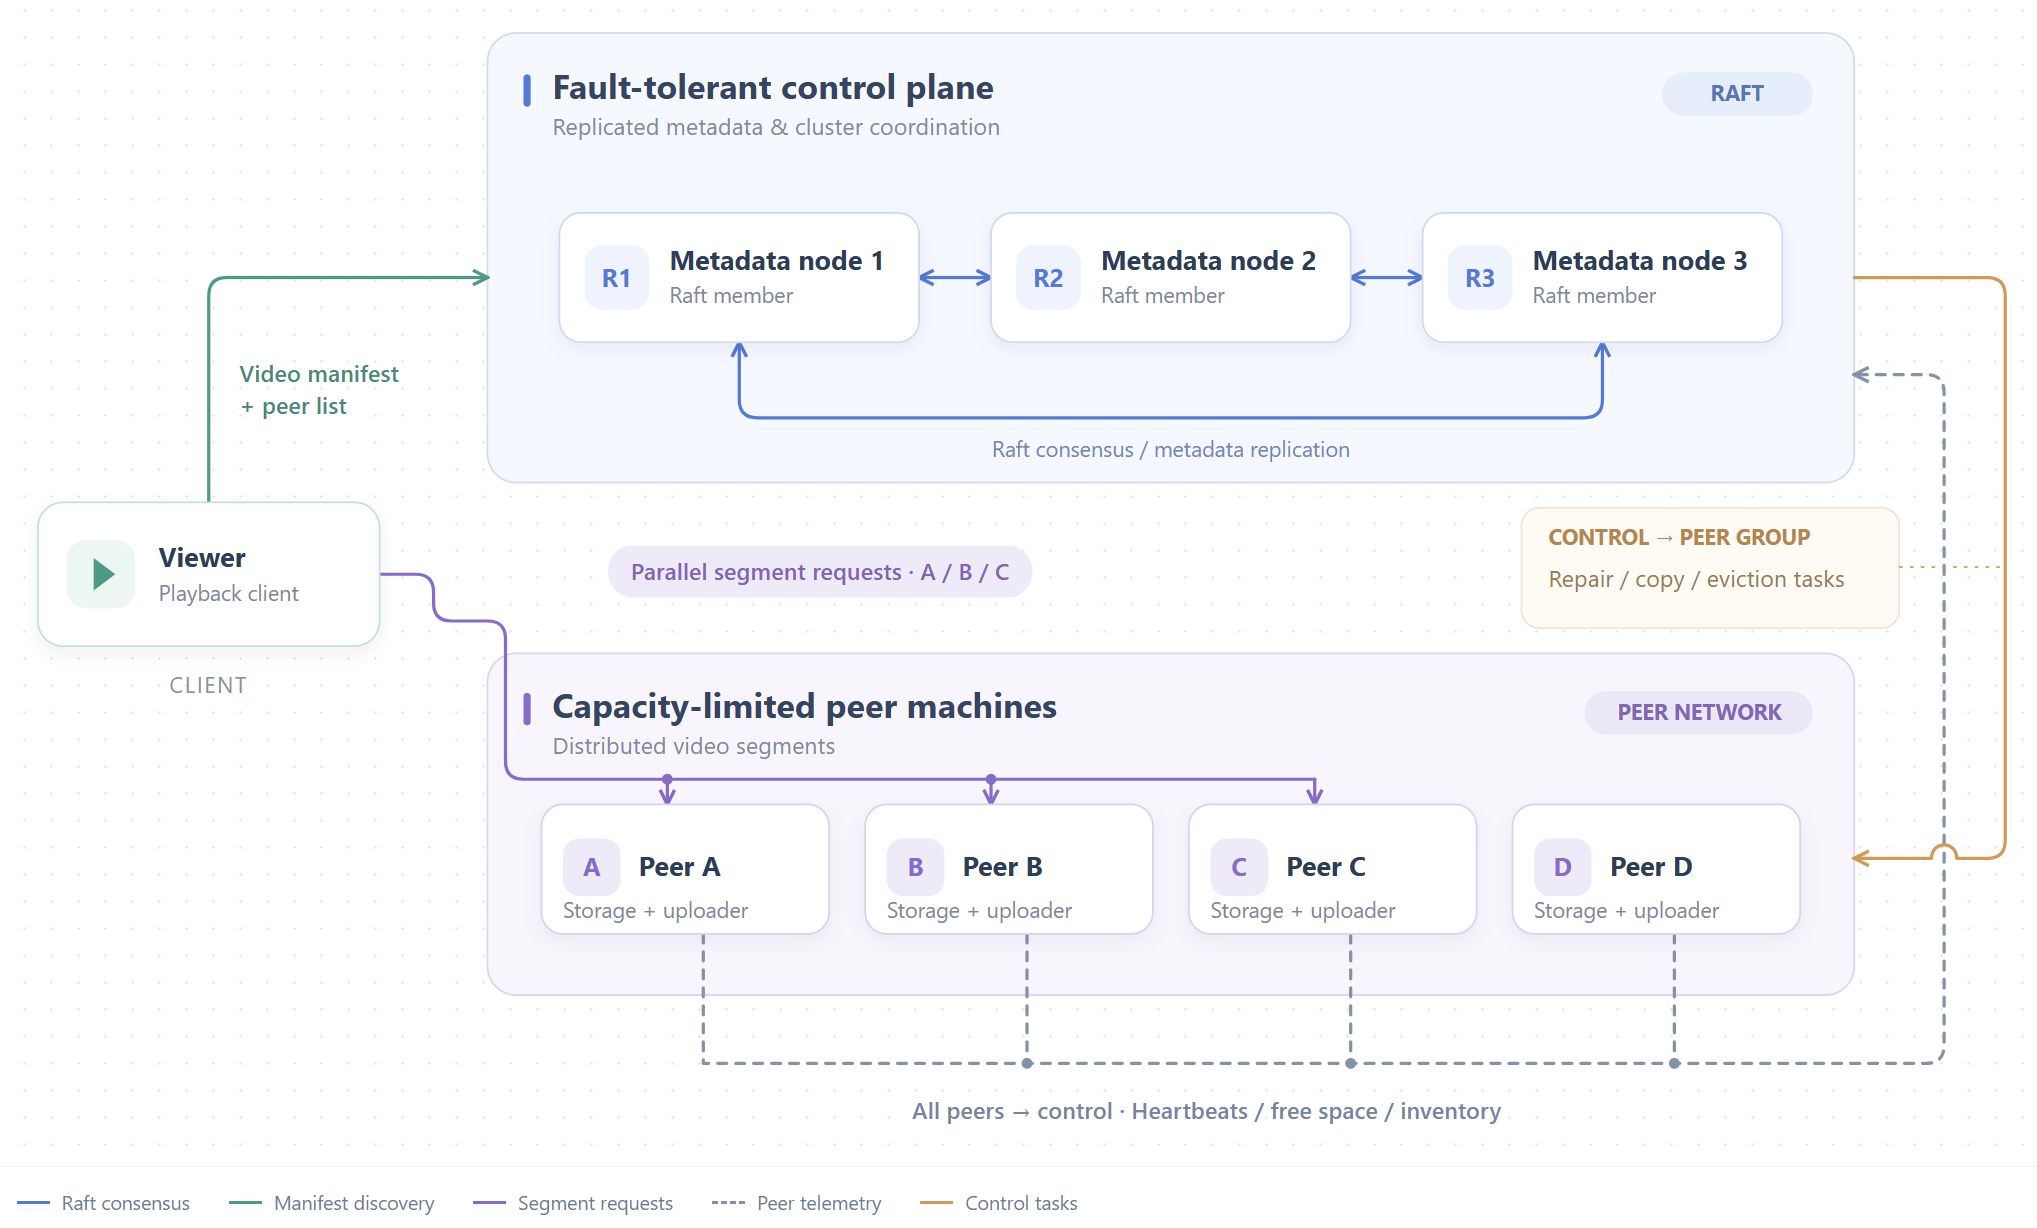
\includegraphics[width=2\linewidth]{assets/architecture.png}
\end{center}
\caption{\label{fig:vectors}System Architecture}
\end{figure}
% %% %---------------------------


% Here's a typical reference to a floating figure:
% Figure~\ref{fig:vectors}. Floats should usually be placed where latex
% wants then. Figure\ref{fig:vectors} is centered, and has a caption
% that instructs you to make sure that the size of the text within the
% figures that you use is as big as (or bigger than) the size of the
% text in the caption of the figures. Please do. Really.

% In our case, we've explicitly drawn the figure inlined in latex, to
% allow this tex file to cleanly compile. But usually, your figures will
% reside in some file.pdf, and you'd include them in your document
% with, say, \textbackslash{}includegraphics.

% Lists are sometimes quite handy. If you want to itemize things, feel
% free:

% \begin{description}
  
% \item[fread] a function that reads from a \texttt{stream} into the
%   array \texttt{ptr} at most \texttt{nobj} objects of size
%   \texttt{size}, returning returns the number of objects read.

% \item[Fred] a person's name, e.g., there once was a dude named Fred
%   who separated usenix.sty from this file to allow for easy
%   inclusion.
% \end{description}

% \noindent
% The noindent at the start of this paragraph in its tex version makes
% it clear that it's a continuation of the preceding paragraph, as
% opposed to a new paragraph in its own right.


% \subsection{LaTeX-ing Your TeX File}
% %-----------------------------------

% People often use \texttt{pdflatex} these days for creating pdf-s from
% tex files via the shell. And \texttt{bibtex}, of course. Works for us.

% %-------------------------------------------------------------------------------
% \section*{Acknowledgments}
% %-------------------------------------------------------------------------------

% The USENIX latex style is old and very tired, which is why
% there's no \textbackslash{}acks command for you to use when
% acknowledging. Sorry.

% %-------------------------------------------------------------------------------
% \section*{Availability}
% %-------------------------------------------------------------------------------

% USENIX program committees give extra points to submissions that are
% backed by artifacts that are publicly available. If you made your code
% or data available, it's worth mentioning this fact in a dedicated
% section.

%-------------------------------------------------------------------------------
\bibliographystyle{plain}
\bibliography{references}

%%%%%%%%%%%%%%%%%%%%%%%%%%%%%%%%%%%%%%%%%%%%%%%%%%%%%%%%%%%%%%%%%%%%%%%%%%%%%%%%
\end{document}
%%%%%%%%%%%%%%%%%%%%%%%%%%%%%%%%%%%%%%%%%%%%%%%%%%%%%%%%%%%%%%%%%%%%%%%%%%%%%%%%

%%  LocalWords:  endnotes includegraphics fread ptr nobj noindent
%%  LocalWords:  pdflatex acks